%%%%%%%%%%%%%%%%%%%
% Import Setting  %
%%%%%%%%%%%%%%%%%%%

\documentclass[
    paper=a4,
    fontsize=12pt,
    parskip=half,
    headheight=32pt,
    DIV=12,
    BCOR=3mm
  ]{scrartcl}

  \usepackage[english, ngerman]{babel}
  \usepackage[utf8]{inputenc}
  \usepackage{amsmath}
  \usepackage{graphicx}
  \usepackage{bookmark}
  \usepackage{array}
  %usepackage{showframe} % to see the frame of the pdf
  \usepackage[a4,center,cam]{crop} % set size of page frame. Synergy with Koma-Script

  % Allows adding inline-code
  \usepackage{listings}

  % Allow direct copy&paste from the pdf
  \usepackage[T1]{fontenc}
  \usepackage[utf8]{inputenc}

  \PassOptionsToPackage{colorlinks=true,linkcolor=blue}{hyperref}
  %\usepackage[colorlinks=true,linkcolor=blue]{hyperref}

  % Header and Footer
  \usepackage[headsepline=0.4pt,plainfootsepline]{scrlayer-scrpage}
  \pagestyle{scrheadings}
  \clearpairofpagestyles

  \ihead{Reverse Engineering}
  \ohead{
\includegraphics[width=2cm]{../img/HM_Logo.jpg}}
  \usepackage{lastpage}
  \cfoot{Seite \pagemark\hspace{0.9pt} von \hspace{0.9pt}\pageref{LastPage}}

\begin{document}

%%%%%%%%%%%%%%%
% Titelseite  %
%%%%%%%%%%%%%%%
\begin{titlepage}
    \newcommand{\HRule}{\rule{\linewidth}{0.35mm}} % Defines a new command for the horizontal lines

    \center% Center everything on the page

    \textsc{\LARGE Reverse Engineering}\\[0.7cm]

    \begin{figure} [!ht]
        \centering
        
\includegraphics[width=5cm]{../img/HM_Logo.jpg}
    \end{figure}

    \textsc{\Large Übung 1 - Gruppe 3}\\[0.7cm]

    \HRule

    \begin{tabular}{*{3}{>{\centering}p{.25\textwidth}}}
        Ludwig Karpfinger & Armin Jeleskovic & Valentin Altemeyer \tabularnewline
        \url{ludwig.karpfinger@hm.edu} & \url{a.jeleskovic@hm.edu} & \url{valentin.altemeyer@hm.edu}
    \end{tabular}\par
    \HRule

    \textsc{}\\[0.3cm]

    \let\endtitlepage\relax

\end{titlepage}

%%%%%%%%%%%%%%%%%%%%%%%%%%%%%%
% Aufgaben ab hier einfügen  %
%%%%%%%%%%%%%%%%%%%%%%%%%%%%%%
\section*{Aufgabe 1 REMnux installieren}
\section*{Aufgabe 2 REMnux Tool Check}

\subsection*{a) Aus welchen Quellen kann ein Tool von REMnux stammen?}
Remnux kann wie jede andere Linux-Distro Software aus den angegebenen Quellen installieren.
(abgesehen von sonstigen Paketmanagern, wie \textit{snap, flatpack, AppImage})
Folgender Befehl zeigt die Repos an:

\begin{lstlisting}[language=bash]
  $ sudo grep -Erh ^deb /etc/apt/sources.list*
\end{lstlisting}
Es fällt auf, dass ein spezielles Remnux Repo vorhanden ist namens:

\mbox{\textit{http://ppa.launchpad.net/remnux/stable/ubuntu}}. Diese Repo wurde durch \textit{remnux.sls} hinzugefügt\footnote{\url{https://github.com/REMnux/salt-states/blob/master/remnux/repos/remnux.sls}}

Die Besonderheit bei Remnux ist, dass der \textit{Remnux Installer} automatisch Software installiert, konfiguriert und aktualisiert.
Die Eigenschaften von Software, wie Download-Quelle, Installation Path, Hashnummer, Rechte, Abhängigkeiten und Configs, werden durch sogenannte \textit{state files} bestimmt.
Diese Files befinden sich auf GitHub und werden durch den \textit{Remnux Installer} geladen.

Remnux nutzt gemäß den Remnux Docs\footnote{\url{https://docs.remnux.org/behind-the-scenes/technologies/debian-packages}} folgende Installationsquellen:
\begin{itemize}
    \item pip
    \item gems
    \item npm
    \item apt Repos
\end{itemize}

\subsection*{b) Welche Tools stammen nicht aus Open Source Quellen?}

Das Github Repo wurde im Ordner \textit{/Documents/} gecloned.

Lösung mit \textit{grep}:

\begin{lstlisting}[language=bash]
$ grep -r --include="*.sls"
> -Eio "source: (http|https)://[a-zA-Z0-9./?=_%:-]*"
> /home/remnux/Documents/salt-states/remnux/
> | grep -v "github"
> | cut -d'/' -f10
> | uniq -u
\end{lstlisting}

Output:
\begin{lstlisting}
    snapshots.mitmproxy.org
    www.netresec.com
    didierstevens.com
    www.nowrap.de
    bitbucket.org
    www.mitec.cz
    www.nowrap.de
    www.cert.at
    www.netresec.com
    www.didierstevens.com
    radare.mikelloc.com
\end{lstlisting}

Erklärung:

Es wird \textit{command-chaining} verwendet.
Das Tool \textit{grep} sucht mittels \textit{regex} nach allen URLs in allen \textit{.sls} files.
Ergebnisse, die den String \textit{github} beinhalten, werden ausgeschlossen.
Der \textit{cut} Befehl filtert beim Output die Domains heraus.
Der \textit{uniq} Befehl eliminiert alle doppelten Ergebnisse.

\newpage

Lösung mit \textit{Yara}:

\begin{figure} [!ht]
\centering
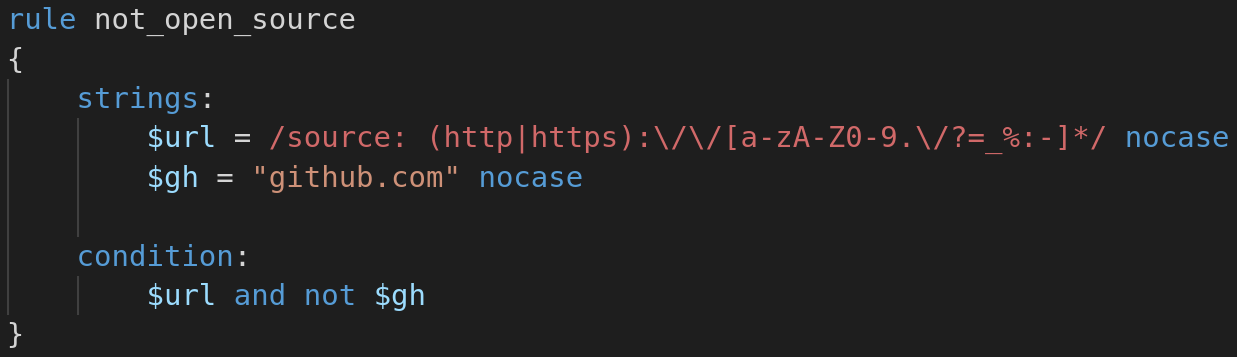
\includegraphics[width=15cm]{../img/yara.PNG}
\end{figure}

Das Github Repo \textit{salt-states-master} wurde in den Ordner \textit{/home/remnux/Desktop/uebung1/} geklont.

Die Regel \textit{not\_open\_source.yara} wurde in der Kommandozeile wie folgt ausgeführt:

\begin{lstlisting}[language=bash]
$ yara -s -r
> not_open_source.yara
> /home/remnux/Desktop/uebung1/salt-states-master
\end{lstlisting}

Die Regel wird rekursiv auf alle Dateien im geklonten Github Repo angewandt (primär \textit{.sls} Dateien). Es werden alle Dateien gefiltert in denen eine Source-URL (\textit{\$url}) enthalten ist, die nicht den String \textit{github.com} (\textit{\$gh}) enthält.

\newpage

\section*{Aufgabe 3 File Classification}

\subsection*{a) samples.zip - not stripped}

\subsubsection*{bin a}

\begin{itemize}
    \item Es handelt sich um eine AMD 64bit ELF Datei im little-endian Format, die durch GCC kompiliert wurde.
    \item Clamscan hat keine bekannten Viren entdeckt.
    \item signsrch hat keine Pattern zur Verschlüsselung, Encoding, Kompression gefunden
    \item Magic Bytes: 7f 45 4c 46 02 01 01 00 00 00 00 00 00 00 00 00
    \item Es handelt sich um den Linux cp Command
\end{itemize}

\subsubsection*{bin b}

\begin{itemize}
    \item Es handelt sich um eine AMD 64bit ELF Datei im little-endian Format, die durch GCC kompiliert wurde.
    \item Der \textit{Unix.Tool.Pnscan-8031486-0} Virus wurde gefunden
    \item signsrch hat keine Pattern zur Verschlüsselung, Encoding, Kompression gefunden
    \item Es handelt sich um den TCP Portscanner Pnscan
\end{itemize}

\subsubsection*{bin c}

\begin{itemize}
    \item Es handelt sich um eine AMD 64bit ELF Datei im little-endian Format, die durch GCC kompiliert wurde.
    \item Der \textit{Unix.Trojan.Mirai-7100807-0} Virus wurde gefunden
    \item signsrch hat keine Pattern zur Verschlüsselung, Encoding, Kompression gefunden
    \item Virus ruft C++ Compiler und Linux Programme, wie Watchdog, auf
\end{itemize}

\subsection*{b) binaries.zip - stripped}

\subsubsection*{bin a Doppelgänger}

Yara file (64 byte Header) == Output \textit{bin 3173}:

\begin{lstlisting}
    rule bin_a
    {
      strings:
        $id0 = {7f 45 4c 46 02 01 01 00 00 00 00 00 00 00 00 00}
        $id1 = {02 00 3e 00 01 00 00 00 d0 25 40 00 00 00 00 00}
        $id2 = {40 00 00 00 00 00 00 00 80 77 02 00 00 00 00 00}
        $id3 = {00 00 00 00 40 00 38 00 09 00 40 00 1f 00 1c 00}
      condition:
        all of them
    }
\end{lstlisting}

\subsubsection*{bin b Doppelgänger}

Yara file (objdump -drS aus .text) == Output \textit{bin 2723}:

\begin{lstlisting}
    rule bin_b
    {
      strings:
        $rcx = {48 c7 c1 90 50 40 00}
        $rdi = {48 c7 c7 60 44 40 00}
        $call = {e8 e7 fd ff ff}
      condition:
        all of them
    }
\end{lstlisting}

\subsubsection*{bin c Doppelgänger}

Yara file (objdump -drS aus .text) == Output \textit{bin 1207}:

\begin{lstlisting}
    rule bin_c
    {
      strings:
        $rcx = {49 c7 c0 80 f3 40 00}
        $rdi = {48 c7 c7 50 c3 40 00}
        $call = {e8 d7 fd ff ff}
      condition:
        all of them
    }

\end{lstlisting}

\section*{Aufgabe 4 - Firmware Identifikation}

\subsection*{a) Dump Analyse}

Die Entropie gibt Aufschluss darüber, dass die Firmware komprimiert und/oder verschlüsselt.
Die Schwachstelle bei der XOR-Verschlüsselung ist diese Formel:
\begin{lstlisting}[language=Python]
    x^0 = x
\end{lstlisting}

Es lässt sich somit das Muster - \textit{88 44 A2 D1 68 B4 5A 2D} - finden.

Über den Hexeditor wird die entschlüsselte Datei als \textit{decrypt.bin} abgespeichert.

\subsection*{b) Extrahieren}

Das Squashfs Filesystem ist xz compressed und 5739914 bytes groß.
\begin{lstlisting}
    $ binwalk decrypt.bin
    $ dd if=decrypt.bin skip=1900672 of=linux bs=1
    $ unsqushfs linux
\end{lstlisting}

Mit dem \textit{dd} Befehl wird die Filesystem Partition herausgeschnitten und schließlich mit unsquashfs decompressed.

\subsection*{c) Gerätetyp und Version}

Die Analyse der Datei \textit{/sbin/dbox init} ergibt, dass es sich wahrscheinlich um einen Router handelt.

Bei der Version von \textit{Squashfs} handelt es sich wahrscheinlich um Version 1.0.0 (hier bin ich mir nicht ganz sicher,
 da ich keine konkrete Versionsangabe gefunden habe)


\end{document}